\chapter{Modelling}
\label{sec:modelling}

This chapter describes the predictive modelling of blood pressure using Random Forest methods. The analysis builds on the cleaned dataset described in Chapter~\ref{sec:eda} ($n = 15{,}219$) and progresses from a baseline multi-output regressor through feature engineering, robustness checks, and a classification extension. Implementation details are documented in \texttt{modeling.ipynb}.

\section{Modelling Pipeline Overview}
\label{sec:modelling_overview}

The pipeline comprises four stages:
\begin{enumerate}
    \item \textbf{Data preparation} --- encode categorical and boolean predictors as numeric features; define systolic and diastolic blood pressure as joint regression targets.
    \item \textbf{Baseline regression} --- train a multi-output Random Forest on demographic and clinical covariates only.
    \item \textbf{Model refinement} --- apply age-stratified splitting, cross-validation, tree-depth tuning, and augment features with temporal and weather variables.
    \item \textbf{Evaluation and extensions} --- compare models on held-out test data; add hypertension classification and residual diagnostics.
\end{enumerate}

The primary modelling goal is to predict measured blood pressure from available covariates. A secondary goal is to classify elevated blood pressure categories when exact mmHg prediction proves unreliable. Model performance is assessed using the coefficient of determination ($R^2$) and mean absolute error (MAE), defined for outcome $y_i$ and prediction $\hat{y}_i$ as
\begin{equation}
    R^2 = 1 - \frac{\sum_{i=1}^{n}(y_i - \hat{y}_i)^2}{\sum_{i=1}^{n}(y_i - \bar{y})^2},
    \qquad
    \mathrm{MAE} = \frac{1}{n}\sum_{i=1}^{n}\left|y_i - \hat{y}_i\right|,
    \label{eq:metrics}
\end{equation}
where $n$ denotes the number of test observations and $\bar{y}$ is the sample mean of the outcome.

\section{Feature Set and Encoding}
\label{sec:modelling_features}

For simplicity, all model inputs are transformed to numeric form. Categorical and boolean variables (gender, smoker status, known blood sugar, known cholesterol, under treatment) are one-hot encoded with \texttt{drop\_first=True}. The baseline predictor set comprises seven features: age, health condition (\texttt{befinden}), gender, smoker status, known blood sugar, known cholesterol, and under treatment. Two blood pressure outcomes are predicted jointly: systolic (\texttt{bp\_systolic}) and diastolic (\texttt{bp\_diastolic}).

\section{Train--Test Splitting}
\label{sec:modelling_split}

The initial baseline used a standard 80/20 split. In the refined pipeline, splitting is \textbf{stratified by age group} (0--20, 21--40, 41--60, 61--80, 81--100 years) to preserve the age distribution across training and test sets (12,175 / 3,044 records). This addresses the concern that a random split could produce unrepresentative test cohorts in a dataset dominated by middle-aged participants.

\section{Weather Data Integration}
\label{sec:modelling_weather}

Hourly temperature and relative humidity for Graz, Austria (2006) are retrieved from the Open-Meteo Historical Weather API \cite{open_meteo} and matched to each measurement timestamp rounded to the nearest hour. One hundred twenty-three records fall outside the weather coverage period and are excluded, leaving $n = 15{,}096$ for weather-enhanced models.

\section{Baseline Model: Multi-Output Random Forest}
\label{sec:modelling_baseline}

The baseline model is a \textbf{multi-output Random Forest regressor} that predicts systolic and diastolic blood pressure simultaneously from the seven baseline features. Hyperparameters are held constant across iterations unless noted:
\begin{itemize}
    \item \texttt{n\_estimators = 500}, \texttt{max\_features = 'sqrt'}, \texttt{min\_samples\_leaf = 5}, \texttt{random\_state = 42}.
    \item Baseline \texttt{max\_depth = None} (unlimited tree depth).
\end{itemize}

On the stratified test set, the baseline achieves weak explanatory power (Table~\ref{tab:model_comparison}). Systolic predictions show a modest positive trend with actual values; diastolic predictions are substantially noisier. Mean absolute errors of 10--14~mmHg are clinically meaningful: a typical prediction may deviate from the true value by an amount relevant to hypertension diagnosis.

Feature importance confirms that \textbf{age dominates} (importance $\approx 0.68$), followed by under treatment ($\approx 0.11$), gender ($\approx 0.08$), and health condition ($\approx 0.06$). Smoker status, blood sugar awareness, and cholesterol awareness contribute least ($< 0.03$ each). Lifestyle and clinical-awareness variables therefore add limited predictive information relative to age.

As a supplementary check, \textbf{single-output models} that include the complementary blood pressure component as a predictor perform substantially better ($R^2 \approx 0.48$--$0.53$). This reflects the strong correlation between systolic and diastolic readings ($r \approx 0.66$) rather than improved prediction from demographic covariates alone. Single-output formulations are not pursued further because they are not applicable when both pressures must be predicted from non-blood-pressure features.

\section{Cross-Validation and Overfitting Control}
\label{sec:modelling_cv}

Five-fold cross-validation on the full feature set yields mean $R^2 = 0.140$ ($\pm 0.013$) for systolic and $0.035$ ($\pm 0.014$) for diastolic blood pressure, confirming that baseline performance is stable across folds rather than an artefact of a single split.

Tree depth is tuned via cross-validation on systolic $R^2$; results are summarised in Table~\ref{tab:depth_tuning}.

\begin{table}[h]
    \centering
    \caption{Cross-validated systolic $R^2$ by maximum tree depth (\texttt{modeling.ipynb}).}
    \label{tab:depth_tuning}
    \begin{tabular}{lc}
        \toprule
        \textbf{Maximum depth} & \textbf{Mean CV $R^2$} \\
        \midrule
        3  & 0.138 \\
        5  & 0.157 \\
        10 & 0.163 \\
        20 & 0.140 \\
        None (unlimited) & 0.140 \\
        \bottomrule
    \end{tabular}
\end{table}

Moderate depth (\texttt{max\_depth = 10}) performs best. Unlimited or very deep trees (\texttt{None}, 20) match shallower cross-validated performance but show signs of overfitting relative to the depth-10 setting. All subsequent refined models use \texttt{max\_depth = 10}.

\section{Temporal Feature Engineering}
\label{sec:modelling_temporal}

Four temporal variables are extracted from the measurement timestamp: hour of day, day of week, month, and season (one-hot encoded). Combined with the baseline covariates, the \textbf{temporal Random Forest} improves test-set performance, with the largest gain for diastolic blood pressure (Table~\ref{tab:model_comparison}).

In the temporal model, age remains the strongest predictor (importance $\approx 0.42$), but hour ($\approx 0.09$), day of week ($\approx 0.08$), and month ($\approx 0.06$) contribute non-trivial information. Permutation importance confirms age as the dominant variable while temporal features provide incremental value.

\section{Weather Feature Engineering}
\label{sec:modelling_weather_features}

Temperature (2~m) and relative humidity (2~m) are added to the temporal feature set. The \textbf{weather-enhanced Random Forest} yields the best regression performance overall, as shown in Table~\ref{tab:model_comparison}.

\begin{table}[h]
    \centering
    \caption{Regression model comparison on held-out test sets (\texttt{modeling.ipynb}).}
    \label{tab:model_comparison}
    \begin{tabular}{lcccc}
        \toprule
        \textbf{Model} & \textbf{Sys.\ $R^2$} & \textbf{Sys.\ MAE} & \textbf{Dia.\ $R^2$} & \textbf{Dia.\ MAE} \\
        \midrule
        Baseline multi-output RF       & 0.130 & 14.14 & 0.042 & 10.50 \\
        Temporal RF                    & 0.176 & 13.81 & 0.086 & 10.19 \\
        Weather-enhanced RF            & 0.192 & 13.60 & 0.097 & 10.05 \\
        \bottomrule
    \end{tabular}
\end{table}

Weather integration reduces mean absolute error by approximately 0.5~mmHg (systolic) and 0.4~mmHg (diastolic) relative to the baseline. The improvement is consistent but modest: even the best model explains only 19\% of systolic variance and 10\% of diastolic variance. Figure~\ref{fig:model_scatter} shows that scatter plots of actual versus predicted values remain widely dispersed.

\begin{figure}[h]
    \centering
    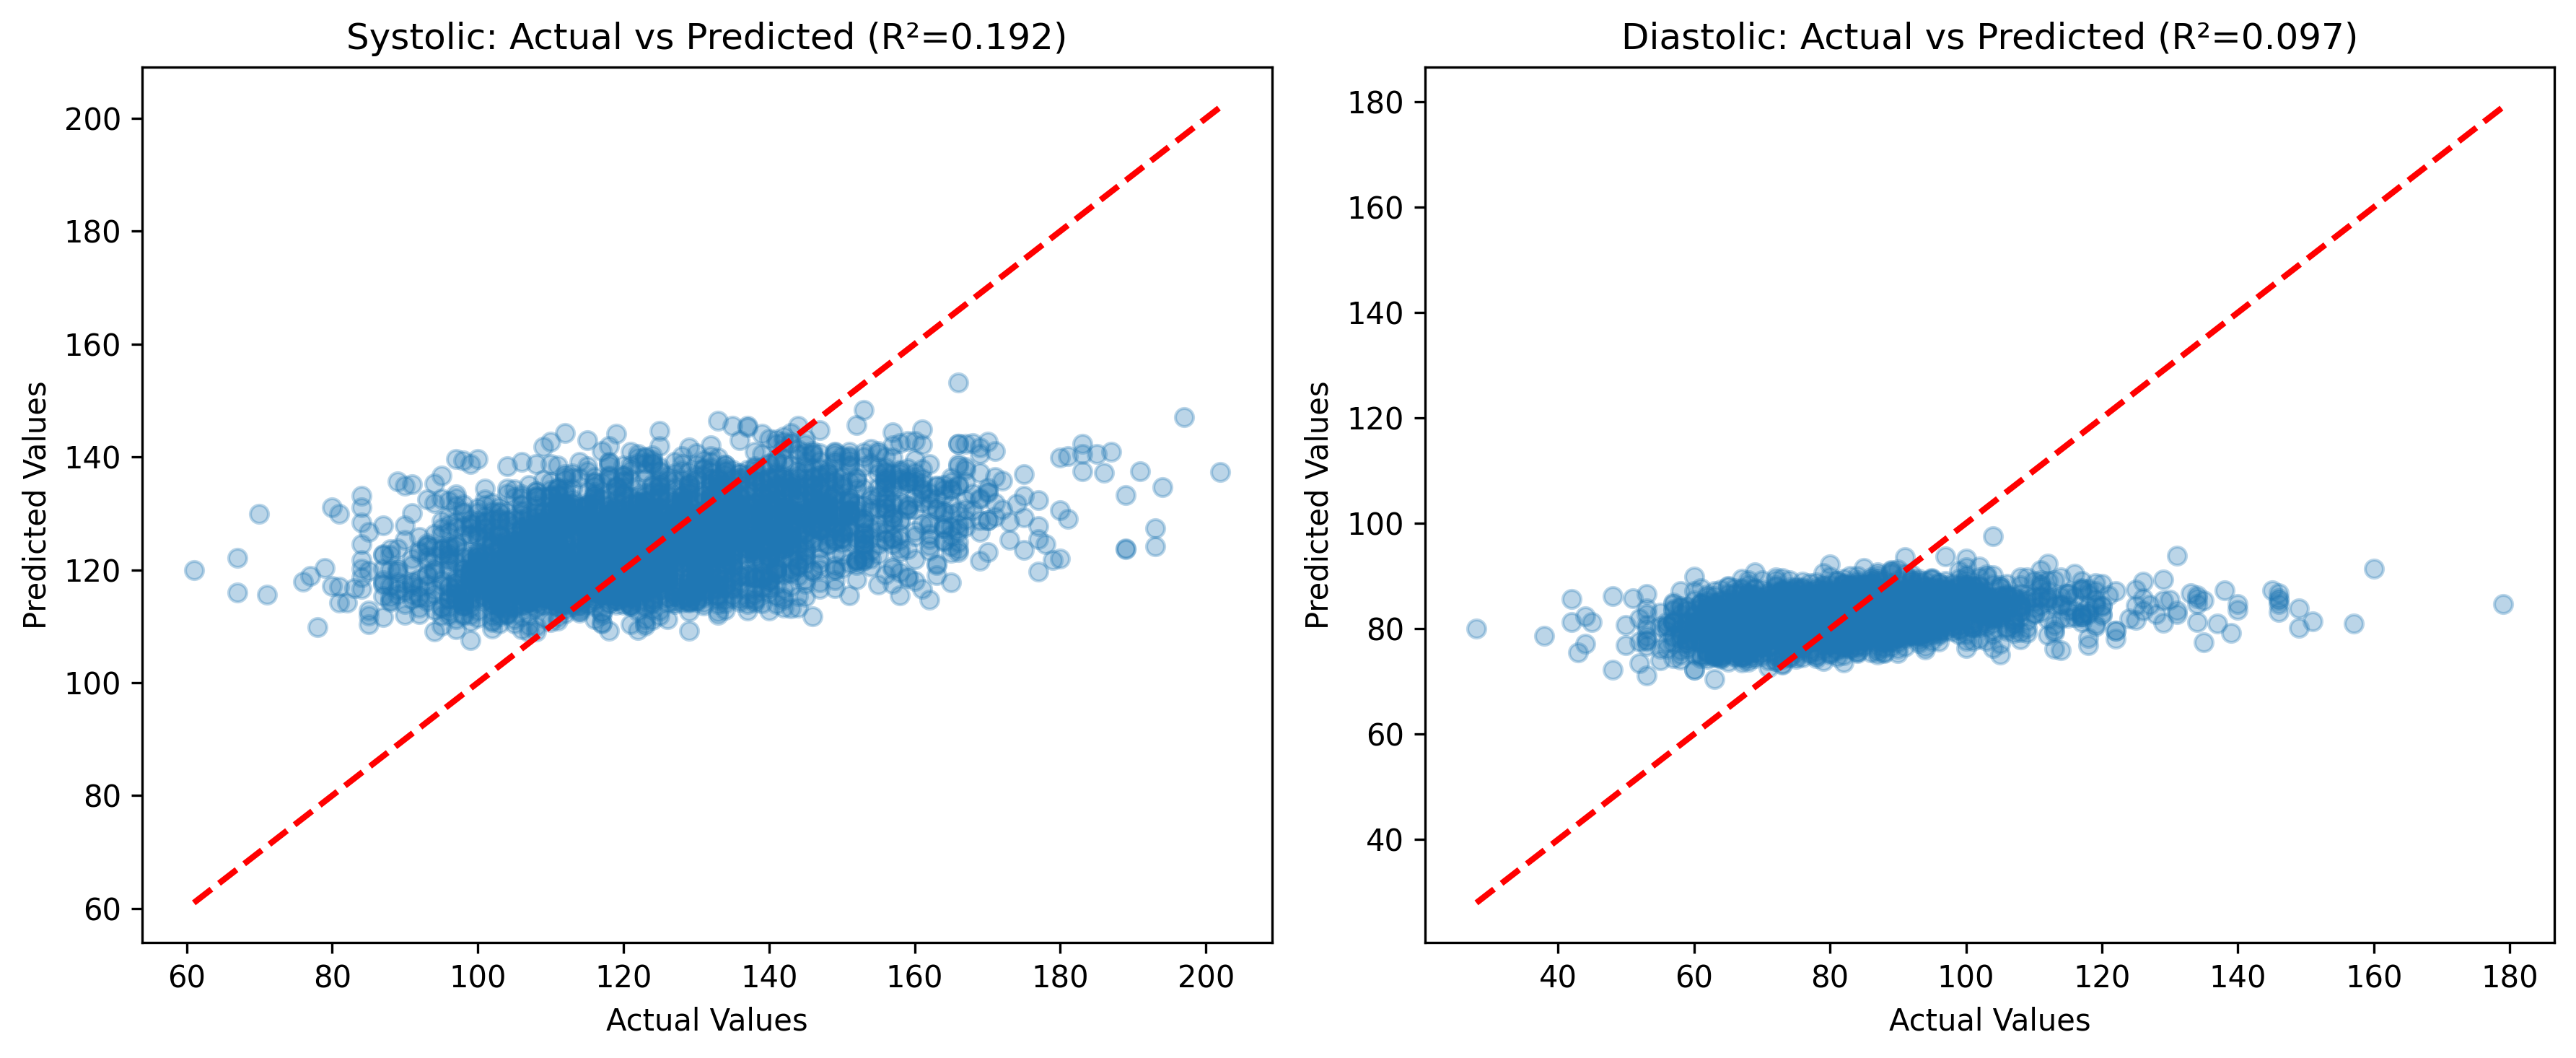
\includegraphics[width=0.85\textwidth]{figures/model_r2_comparison.png}
    \caption{Actual versus predicted blood pressure for the weather-enhanced Random Forest on the held-out test set. Dashed lines indicate perfect prediction.}
    \label{fig:model_scatter}
\end{figure}

Figure~\ref{fig:feature_importance} confirms that age remains the dominant predictor in the weather-enhanced specification; temporal and weather variables provide supplementary information but do not overturn the age gradient.

\begin{figure}[h]
    \centering
    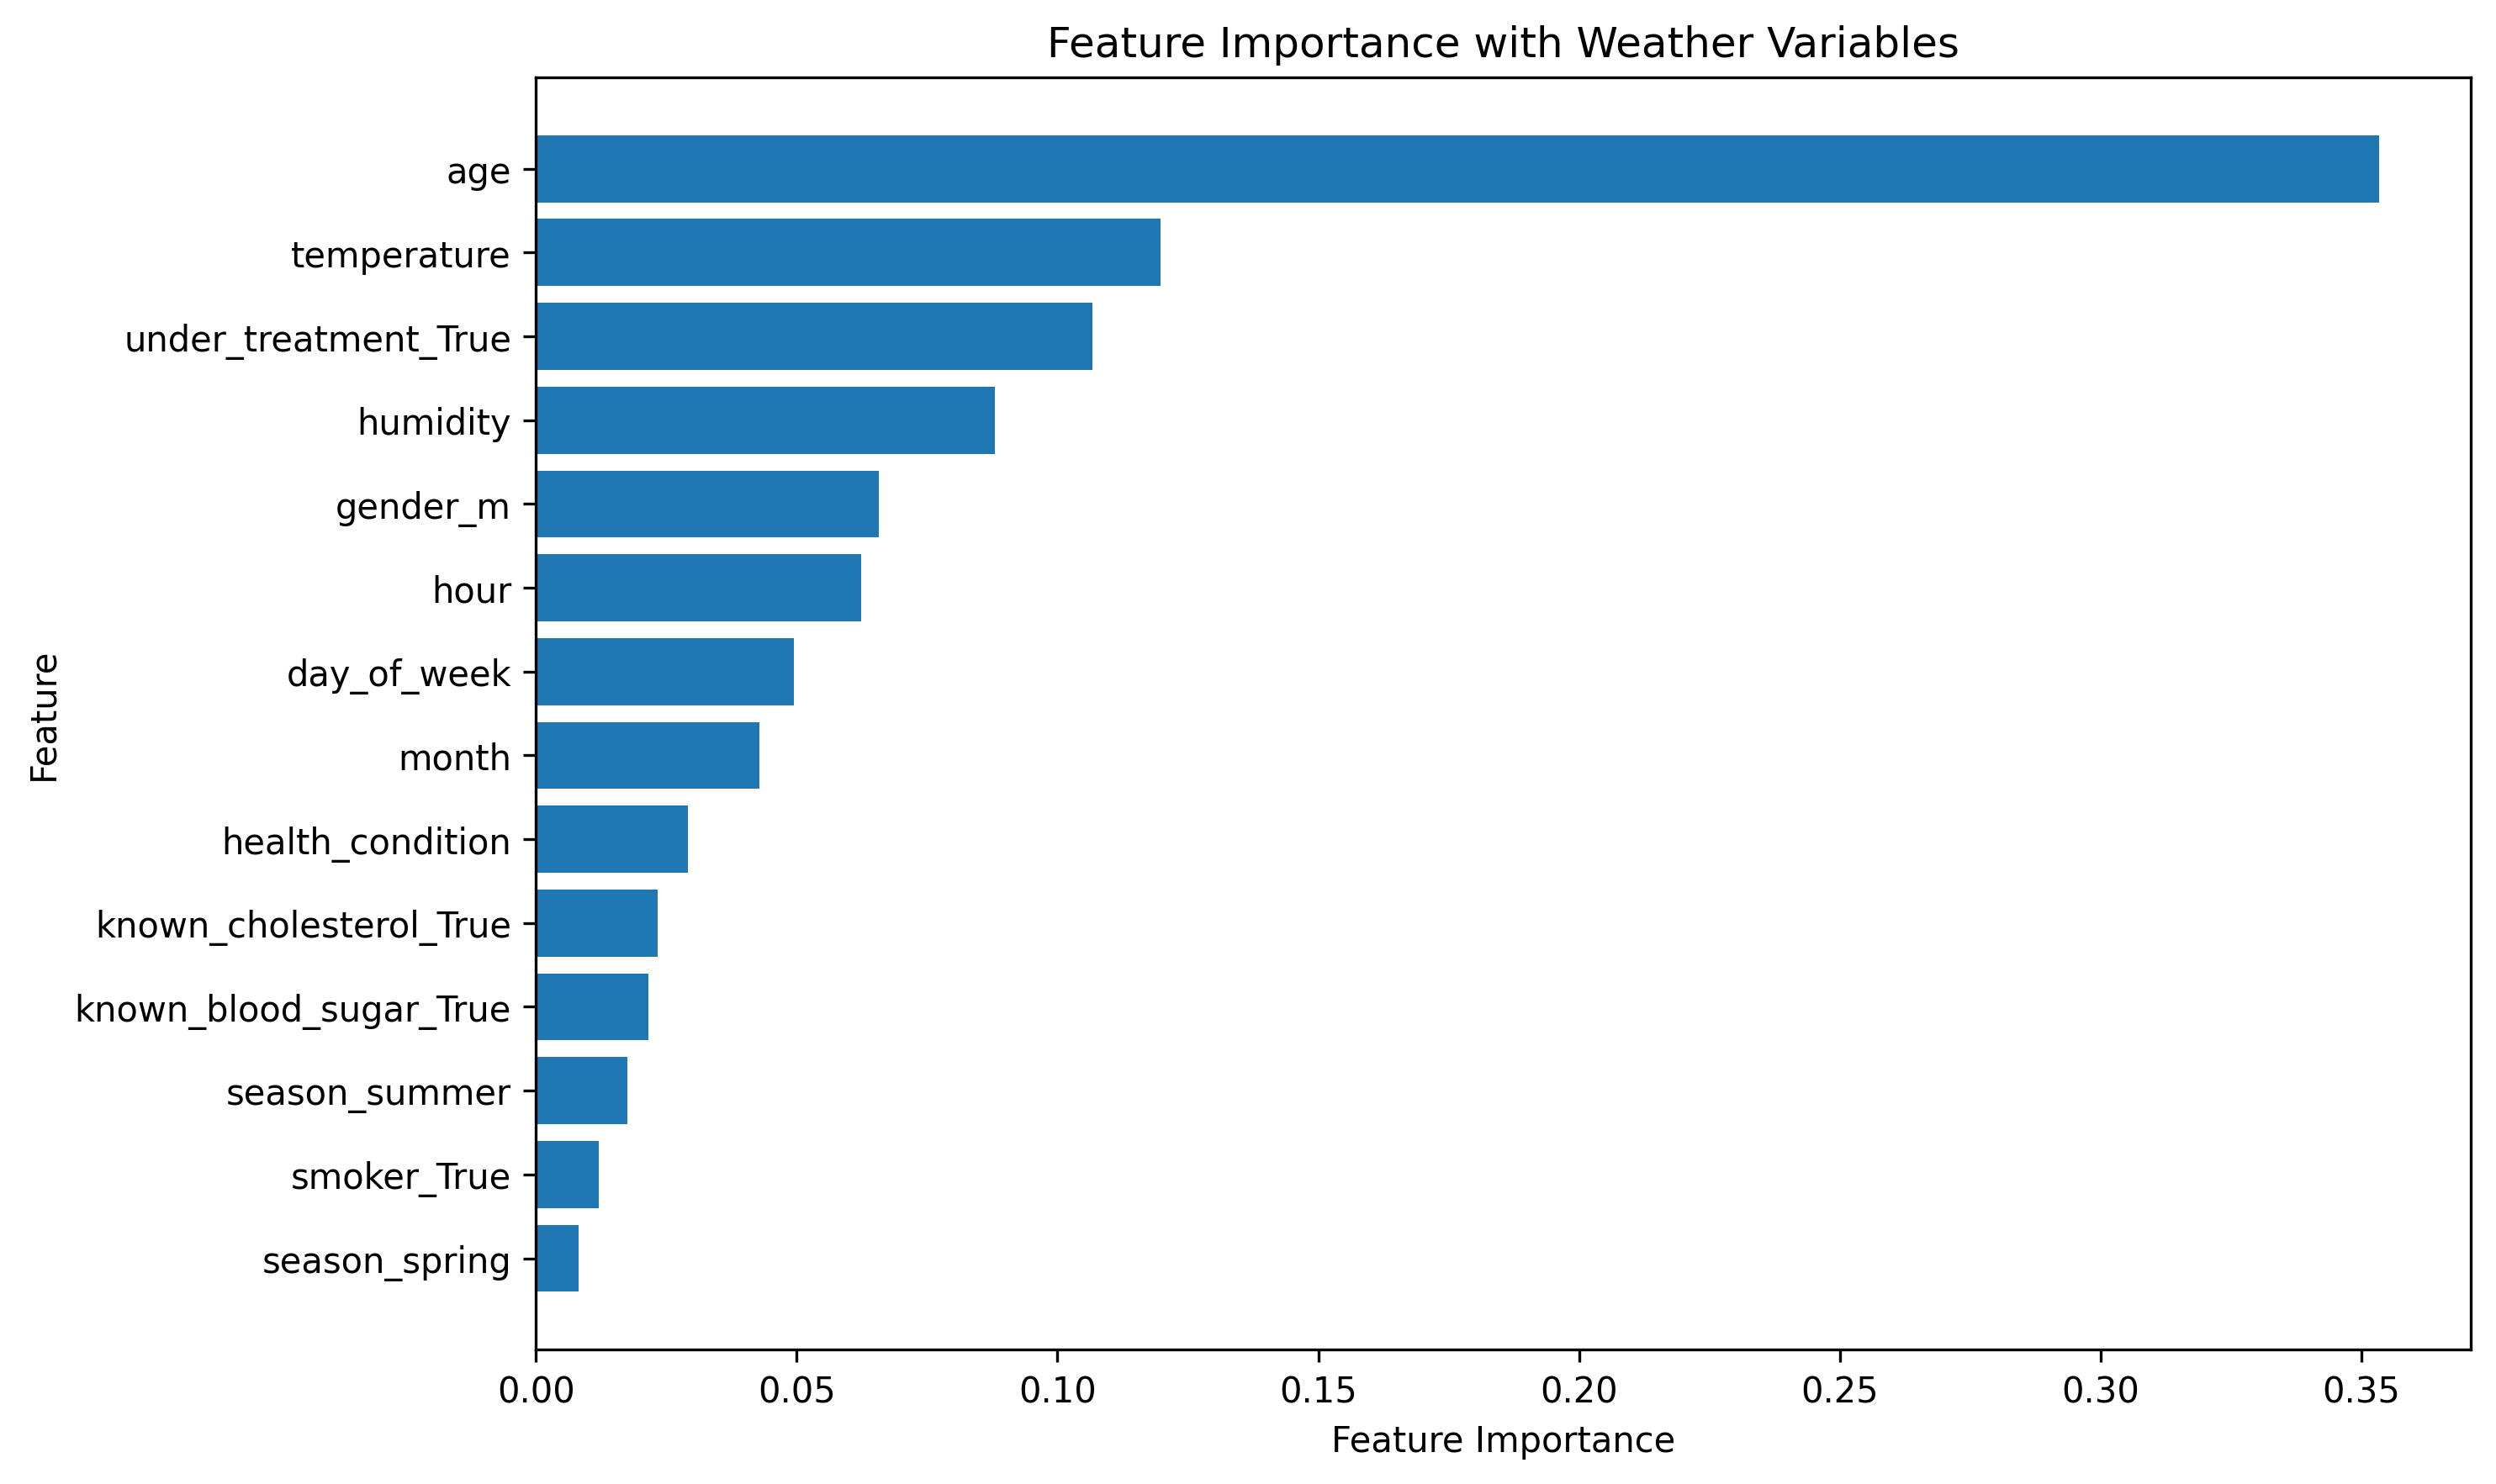
\includegraphics[width=0.75\textwidth]{figures/feature_importance_weather.png}
    \caption{Permutation-based feature importance in the weather-enhanced Random Forest (\texttt{modeling.ipynb}).}
    \label{fig:feature_importance}
\end{figure}

Scenario simulations with the weather-enhanced model hold all covariates fixed except one variable. Predicted blood pressure shows a weak inverse association with temperature and modest within-day variation by hour. These patterns are \textbf{predictive associations}, not evidence of causal effects.

\section{Classification Extension}
\label{sec:modelling_classification}

Elevated blood pressure is defined as systolic $\geq 140$~mmHg or diastolic $\geq 90$~mmHg. Separate binary targets are constructed for systolic and diastolic elevation. A weighted Random Forest classifier (\texttt{class\_weight = 'balanced'}) addresses class imbalance. Features match the weather-enhanced regression model; splitting is stratified on the classification target. Performance on held-out test data is summarised in Table~\ref{tab:classification}.

\begin{table}[h]
    \centering
    \caption{Hypertension classification performance on held-out test data (\texttt{modeling.ipynb}).}
    \label{tab:classification}
    \begin{tabular}{lcccc}
        \toprule
        \textbf{Target} & \textbf{Accuracy} & \textbf{Precision} & \textbf{Recall} & \textbf{F1} \\
        \midrule
        Systolic ($\geq 140$~mmHg) & 0.712 & 0.394 & 0.560 & 0.463 \\
        Diastolic ($\geq 90$~mmHg)  & 0.640 & 0.367 & 0.519 & 0.430 \\
        \bottomrule
    \end{tabular}
\end{table}

Systolic classification achieves higher accuracy and F1, but both targets exhibit \textbf{low precision} (39\% and 37\%). The classifiers detect a reasonable share of elevated cases (recall 52--56\%) at the cost of many false positives. Figure~\ref{fig:threshold} shows that lowering the classification threshold from 0.5 to 0.4 increases recall and F1 slightly, while further reduction trades precision for additional false alarms. The choice of threshold therefore depends on whether false negatives or false positives carry greater cost in the intended application.

\begin{figure}[h]
    \centering
    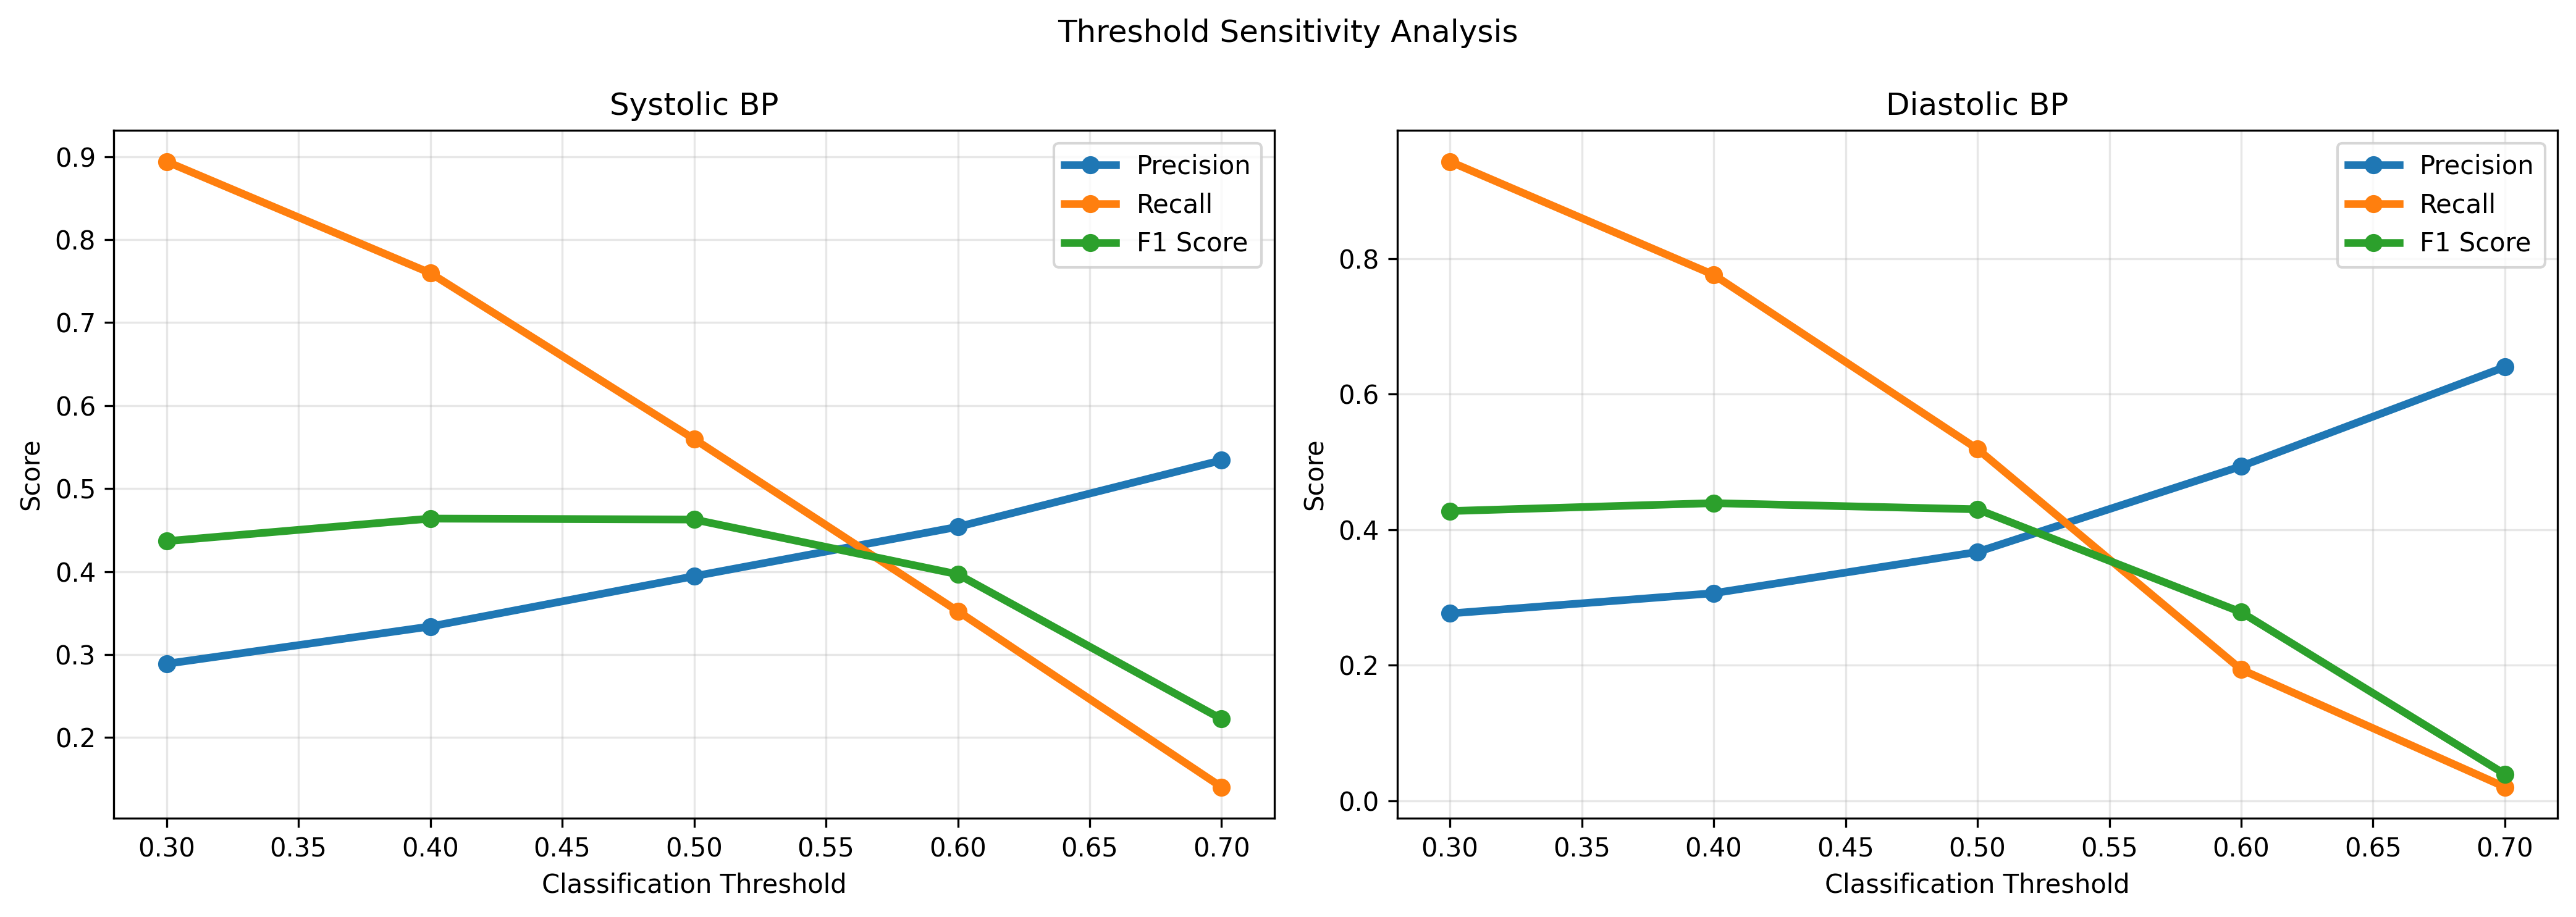
\includegraphics[width=0.85\textwidth]{figures/threshold_sensitivity.png}
    \caption{Precision, recall, and F1 score across classification thresholds for systolic and diastolic hypertension targets (\texttt{modeling.ipynb}).}
    \label{fig:threshold}
\end{figure}

\section{Residual Diagnostics}
\label{sec:modelling_residuals}

Residuals from the weather-enhanced regression model are examined to identify systematic prediction failures. Residuals are approximately centred across temperature values, indicating no strong temperature-related bias. Systolic residuals exhibit larger variance than diastolic residuals, particularly for middle-aged and older participants, suggesting that age-related heterogeneity remains even after modelling.

\section{Summary and Interpretation}
\label{sec:modelling_summary}

The modelling analysis yields three principal conclusions:
\begin{itemize}
    \item \textbf{Limited predictive power.} Available covariates explain a small fraction of blood pressure variance. The best regression model achieves $R^2 = 0.19$ (systolic) and $0.10$ (diastolic), with mean errors of 10--14~mmHg. Models capture population-level trends---especially the age--blood pressure relationship---more reliably than individual readings.
    \item \textbf{Age dominates; refinements add modest value.} Age accounts for most feature importance in every model specification. Temporal and weather features improve performance consistently but do not overturn the dominance of age. Tree-depth tuning and stratified splitting improve methodological rigour without fundamentally changing this conclusion.
    \item \textbf{Classification offers a complementary perspective.} Hypertension classifiers achieve moderate accuracy (64--71\%) but low precision, reflecting both class imbalance and limited feature informativeness. They are better suited to risk stratification than to precise clinical diagnosis.
\end{itemize}

These results complement the inferential findings in Chapter~\ref{sec:eda}. Random Forest and OLS approaches converge on age and treatment status as the strongest associations, while lifestyle variables contribute comparatively little to prediction.
